% ...
% Castellini, Gruppioni, Davalli, Sandini
% submitted to Journal of Physiology, Paris
%
% March, 2009

\documentclass[review,12pt]{elsarticle}

\usepackage{times}
\usepackage{epsfig}
\usepackage{graphicx}
\usepackage{amsmath}
\usepackage{amssymb}
\usepackage{url}

\def\RR{\mathbb{R}}
\def\NN{\mathbb{N}}
\def\xx{\mathbf{x}}
\def\yy{\mathbf{y}}
\def\ww{\mathbf{w}}

\journal{J Physiol Paris}

\begin{document}

\begin{frontmatter}

\title{Advanced hand prosthetics by EMG-based\\
grasp pattern classification and force estimation}

\author[liralab]{Claudio Castellini\corref{corauth}}
\ead{claudio.castellini@unige.it}
\author[inail]{Emanuele Gruppioni}
\ead{e.gruppioni@inail.it}
\author[inail]{Angelo Davalli}
\ead{a.davalli@inail.it}
\author[iit]{Giulio Sandini}
\ead{giulio.sandini@iit.it}

\address[liralab]{LIRA-Lab, University of Genova,
  viale F. Causa 13, 16145 Genova (Italy)}
\address[inail]{INAIL Centro Protesi,
  via Rabuina 14, 40054 Vigorso di Budrio (Bologna, Italy)}
\address[iit]{RBCS Department, Italian Institute of Technology,
  via Morego 30, 16163 Genova (Italy)}

\cortext[corauth]{Corresponding author}

\begin{abstract}
  The dexterity of active hand prosthetics is limited not only due
to the limited availability of dexterous prosthetic hands, but
mainly due to limitations in interfaces. How is an amputee
supposed to command the prosthesis what to do (i.e., how to grasp
an object) and with what force (i.e., holding a hammer or grasping
an egg)? So far, in literature, the most interesting results have
been achieved by applying machine learning to forearm surface
electromyography (EMG) to \emph{classify} finger movements; but
this approach lacks, in general, the possibility of quantitatively
determining the force applied during the grasping act.

In this paper we address the issue by applying machine learning to the
problem of \emph{regression} from the EMG signal to the force a human
subject is applying to a force sensor. A detailed comparative analysis
among three different machine learning approaches (Neural Networks,
Support Vector Machines and Locally Weighted Projection Regression)
reveals that the type of grasp can be reconstructed with an average
accuracy of $90\%$, and the applied force can be predicted with an
average error of $10\%$N, corresponding to about $5$N over a range of
$50$N. None of the tested approaches clearly outperforms the others,
which seems to indicate that machine learning as a whole is a viable
approach.
%
%Notwithstanding the well-known bad conditioning of the surface EMG
%signal then, this looks highly encouraging in applying machine
%learning to enable amputees gain a fine control over advanced
%prosthetic hands, also since a surface EMG setup can be cheaply and
%easily realised and it is totally non-invasive.

\end{abstract}

\begin{keyword}
  learning and adaptive systems \sep
  support vector machines \sep
  hand prosthetics \sep
  electromyography \sep  
\end{keyword}

\end{frontmatter}

\section{Introduction}
\label{sec:intro}
\section{Introduction/Motivation}
\label{sec:intro}

\dropcap{A}utomatic speech recognition (ASR) is the ability of a machine
to convert human speech, coded as an audio signal, into words.
Potential applications of ASR range from human-computer interfaces
to informatics for the disabled to data mining in large speech corpora.
Despite decades of research, state-of-the-art ASR
systems still need to be trained upon very large and heterogeneous data sets
to account for speech variability.
%, or upon a single speaker's speech in controlled conditions.
And nevertheless, human beings show an excellent ability
of understanding one another's speech, independently of the speaker, the
accent, the pitch and speed, noise, etc.

Recent neuroscientific
evidence indicates that the brain motor areas responsible for producing labial
and dental phonemes are also involved in their perception; D'Ausilio et al. \cite{dausilio}
show that in a discrimination task of /b/,/p/,/d/ and /t/, trans-cranial magnetic
stimulation of the lips and tongue \emph{motor areas} creates a bias in favor
of the \emph{perception} of labials, and similarly, stimulation of the tongue
favors dentals. This suggests that motor information may be paramount for
understanding speech in humans.

Inspired by these finding, in this paper we investigate whether the knowledge of speech production in humans 
integrated into an automatic phoneme classifier improves the identification in the acoustic dimension 
of the specific behaviors of the /b/,/p/,/d/ and /t/ plosive consonants.
 
In ASR, approaches that combine explicit speech production knowledge and audio features
have been proposed (see \cite{king} for a review) as alternatives 
to the classic approach  in which the complex acoustic effects of speech production variability 
(e.g., due to speaking rate) and coarticulation (the phenomenon by which the phonetic realization of a phoneme is affected by its phonemic context) are directly and implicitly modeled in the acoustic domain.

%Although conclusions on the actual utility of speech production knowledge are somehow contradictory

By limiting our investigation on the utility of motor information to the much simpler (than ASR) task of four consonants classification\footnote{Note that a recognition task requires both segmentation of speech into phones and their classification.} we are able to relax working assumptions and avoid technical difficulties that so far have hampered a satisfactory integration of motor information into ASR systems. 

Additionally, from previous work it is not feasible to properly identify which aspects of the recognition process benefit from motor information. For example, motor knowledge may improve the modeling (and so the identification) of coarticulation effects that are seen in the training data set, but not necessarily improve the recognition of phonemes in unseen contexts, i.e., it may not necessarily improve the generalization ability of the ASR system. On the other hand the experimental setup we have designed has the main goal of investigating whether motor information improves the generalization ability of a phoneme classifier.  

%Although the integration of speech production knowledge in an ASR system often brings some improvements, %it is commonly held that the potential of speech production knowledge is far from being exhaustively exploited.  

To this end, we have focused on the automatic version of
the problem tackled in D'Ausilio et al.'s work. For each consonant,
a corresponding typical phonetic motor invariant (MI) was
identified according to basic physiology of speech;
e.g., a fast, voiced opening (plosion) of the lips for /b/, and so on.
MIs were then used to semi-automatically segment the audio/motor data found in a
database of speech/motor trajectories recorded from $6$ subjects.

Subsequently, a simple regression method (namely, a feed-forward neural network) was employed
to build an Audio-Motor Map (AMM), which converts audio features of the isolated segment to
features of the related MI. On an abstract level, an AMM is a mathematical proxy of a mirror
structure \cite{umilta-01}, reconstructing the distal speaker's speech production act while
listening to the related piece of speech.

To test the approach, we have devised three experiments involving a 
classifier in the form of a Support Vector Machine \cite{BGV92}. We wanted to check whether
the use of MI-based features, either those recorded in the database (the ``real''
motor features) or the AMM-reconstructed ones (a more ecological scenario),
could improve the classifier's performance. Our results show that this is the case,
especially when the classifier is trained on incomplete data sets such as 
per-speaker (e.g., training on speakers $1,2,3$ and testing on $4$) and
per-coarticulation(e.g., training on /ba/, /be/, /bi/, /bo/ and testing on /bu/); or when noise is added,
in which case motor features significantly help classification, even when added to a
state-of-the-art set of audio features about $20$ times larger than that extracted
from the MIs.

\subsection{Related Work}

It is known since the Sixties \cite{liberman1} that the audio signal of speech
cannot be effectively segmented down to the level of the single phoneme,
especially as far as stop consonants such as bilabial plosives
are concerned; in particular, their representations in the audio domain are
radically different according to the phoneme which immediately follows.
It remains an open question then, how humans can
distinctly perceive a common phoneme, e.g.,/b/ in  /ba/ and /bi/, since they
apparently have access to the speaker's audio signal only.

The explanation put forward by the so-called motor theory of speech perception
(MTS, \cite{liberman2,galant}) is that, while perceiving sounds,
humans reconstruct \emph{phonetic gestures}, the physical acts of
producing the phonemes, as they were trained since birth to associate
articulatory gestures to the sounds they heard. 

Even ignoring the motor theory of speech perception the use of speech production knowledge is appealing in that the coupling of articulatory and audio streams allows for explicit models of the effects of speech production phenomena (e.g., coarticulation) on the acoustic domain. These effects cannot be precisely modeled (e.g., when the phoneme /a/ affects the phonetic realization of /b/ in /ba/?)  or modeled at all (e.g., what happens when I utter a /o/ with exaggeratedly open jaw?) when the phonemic stream is directly mapped onto the acoustic dimension as in the standard approach to ASR.  

Different solutions have been proposed to integrate speech production knowledge into an ASR system and different types of speech production information has been used, ranging from articulatory measurements (see \cite{zlokarnik,stephenson,wrench}, for example) to symbolic non-measured representations of articulatory gestures that "replicate" a (symbolic) phoneme into all its possible articulatory configurations\footnote{Articulatory configurations are configurations of the positions of the phonetic articulators} (see \cite{richardson, livescu}, for example).
 
   
%One possible reason why ASR is so difficult is then that
%machines have in general no access to the motor representation of the
%audio signal they are supposed to understand. We hypothesize that motor 
%information might help ASR, especially when tests on different speakers and different
%coarticulations are performed: for example, when training on subject $A$ and
%testing on subject $B$, or when training on pseudo-words such as /ba/, /bi/,
%/be/ and then testing for the presence of /b/ in /bo/, /bu/ or even /br/.

Although some studies have shown increased word recognition accuracy when including speech production knowledge in ASR, it is commonly held that the potential of speech production knowledge is far from being exhaustively exploited. Limits of current approaches include: the use of the phoneme as basic unit (as opposed to articulatory configuration, for example) which appears to be too "coarse", especially in the context of spontaneous spoken speech 
%where coarticulation effects are more frequent and marked
;and  the lack of a mechanism that accounts for the different importance of articulators in the realization of a given phoneme (e.g., in the generation of phoneme /b/ lips are critical, i.e., important, while tongue is non-critical).

The traditional approach in which the speech signal is segmented into phones, often referred to as "beads on a string" approach, poses problems to an accurate modeling of spontaneous speech where coarticulation phenomena such as phone deletion or assimilation (where a phone assimilates some articulatory gestures of the preceding/following phone), are frequent and not always predictable and call for finer-grained basic units (see \cite{ostendorf})). To partly make-up for such limitation we propose an alternative approach where, instead of segmenting the audio stream looking at audio features only and then observing the articulatory gestures within the identified phones, we give priority to the motor information in that speech is segmented by searching for phone-specific patterns of the (critical) articulatory gestures.

%Concerning the necessity of a phoneme dependent distinction between critical and non-critical articulators we do not 
%Traditionally (e.g., \cite{bourl,salvi}), the audio speech signal is segmented with a
%fixed-length Hamming window, usually 20ms. long. The resulting sequence
%is then analysed in the frequency or cepstral domain and the
%resulting coefficients are used as features for a classification system.
%One negative aspect of this approach is that it
%neglects the qualitative overall characteristics of the
%phoneme being uttered: depending on the speed of the speech, a consonant
%can have different lengths and, by using the above approach, global
%information about it is lost (see \cite{ostendorf}, where this approach is
%dubbed ``beads-on-a-string''). Nevertheless, as far as we know, there is
%so far no widely accepted alternative method for speech segmentation,
%if the audio signal is the only one available. One attempt, but not based
%upon articulatory data atl all, appears in \cite{bourlard}.


During recognition, articulatory gestures have to be recovered 
from audio information as audio is the only signal available.
Reconstruction of articulatory features has been attempted since a long
time, but in most cases it is not derived from articulatory \emph{data}
gathered from human subjects. One pioneeristic case is that of Papcun
et al. \cite{papcun} where the AMM is carried out by a Multilayer Perceptron.
Our procedure for building the AMM is deeply inspired by this work.
%By using a Multilayer Perceptron we implicitly assume that all articulators have the same importance and that the AMM is a %one-to-one mapping.   
%Papcun et al. \cite{papcun} observed that non-critical articulators have higher variance (in terms of position) than critical %articulators. 
The Multilayer Perceptron tries to carry out the best recovery of all articulatory gestures while more emphasis to the recovery of the gestures of the critical articulators should be given to the detriment of the non-critical articulators, which have higher variance (in terms of position, see \cite{papcun,rose}). Although we do not address this issue, the simple fact that we only consider two articulators alleviates a problem that would be otherwise far more relevant if all articulators were taken into account\footnote{The higher variance of the non-critical articulators is the main cause that makes AMM a one-to-many mapping: different articulatory configurations result in the same acoustic realization. Solutions to properly address this "ill-posed" nature of the AMM have been proposed by Richmond et al. \cite{richmond} and Toda et al. \cite{toda}. }.

%and subsequently Korin Richmond's work
%\cite{richmond2002,richmond2007} who have been able to reconstruct point-by-point
%the trajectories of articulators from the audio signal to a remarkably low
%error rate. The procedure for building the AMM is deeply inspired by their
%work.

Interestingly, the idea of using information about the mechanisms involved in the production of a human action to improve its classification/recognition (in a domain different from the production domain) has not only been applied in the context of speech recognition. For example Metta et al. \cite{metta-06} and Hinton \cite{hinton-2006} 
have shown that articulatory data can improve classification accuracy in automated hand action classification.

%TODO  
% Transferring the method to speech perception seems
% like a natural choice.


\section{Materials and Methods}
\label{sec:m&ms}
%% To test the effectiveness of the approach we recruited $10$ healthy
%% subjects and recorded a dataset of more than $1200$'' of EMG and force
%% signals per subject.

\subsection{Subjects and setup}

%The experiment was carried out on 
We acquired data from ten healthy subjects, two women and eight men,
nine right-handed and one left-handed, of an average age of $30.9 \pm
8.45$ years. The subjects were generally na\"\i ve with respect to the
%experiment.
recording procedure. We placed on each subject's dominant forearm $7$
surface EMG electrodes. The number of electrodes and their positions
were chosen, visually and by palpation, according to the medical
literature \cite{Kendall}. This procedure allowed us
%in order 
to identify the most relevant flexor and extensor muscles of the
forearm, and to record their EMG activity from the spots that should
be least affected by signal cross-talk\footnote{But notice that some of the
aforementioned muscles are deep into the forearm, so that muscle
cross-talk cannot be completely avoided.}. The chosen locations were:

\begin{itemize}

  \item on the forearm ventral side: near the wrist, above the
     \emph{flexor pollicis longus}; centrally, above the \emph{flexor
     digitorum superficialis}; near the elbow, above the \emph{flexor
     digitorum profundus}; and near the wrist, above the \emph{flexor
     digitorum superficialis} again;

  \item on the forearm dorsal side: near the wrist, above the
     \emph{extensor pollicis brevis/abductor pollicis longus};
     centrally, above the \emph{extensor digitorum communis} and
     \emph{extensor digiti minimi}.

\end{itemize}

%\begin{figure*}[!t] \centering
%  \begin{tabular}{ccc}
%    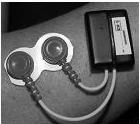
\includegraphics[height=0.16\textheight]{figs/Electrode} &
%    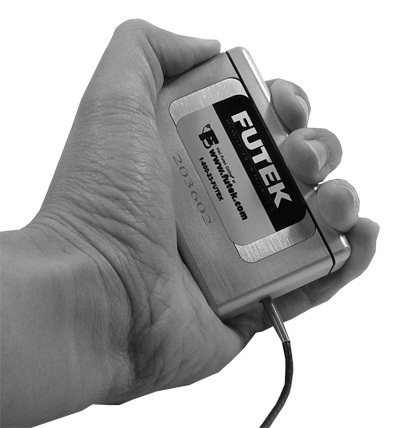
\includegraphics[height=0.16\textheight]{figs/Hand_Gripper} &
%    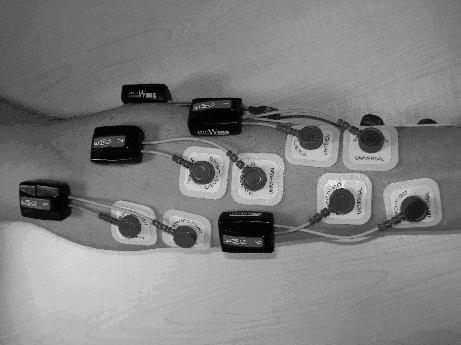
\includegraphics[height=0.16\textheight]{figs/El_Arrangement} \\
%    $(a)$ & $(b)$ & $(c)$ \\
%  \end{tabular}
%  \caption{The experimental setup (\textit{subject side}): $(a)$ an EMG
%    wireless electrode; $(b)$ the FUTEK force sensor; $(c)$ the typical
%    placement of the EMG electrodes on a subject's forearm (ventral side).}
%  \label{fig:SubjSetup}
%\end{figure*}

We employed the electrodes Aurion ZeroWire wireless EMG electrodes
%electrodes (see 
\cite{zerowire}. 
%The use of wireless electrodes helped the subjects
%freely move, to mimic their Daily-Life Activities (DLAs) during the
%acquisition.
%, not beeing wrapped in a thick net of electric cables. 
Moreover the subjects were given a FUTEK LMD500 Hand Gripper force
sensor \cite{LMD500} in order to measure the force applied by her/his
hand during the recording.

%Figure \ref{fig:SubjSetup} shows $(a)$ a single electrode, glued to the subject's forearm skin; $(b)$ the force sensor as gripped during a power grasp; and $(c)$ the typical placement of the electrodes (ventral side of the forearm).

We used a standard National Instruments data acquisition board
(NI-USB6211) connected to the receiver of the EMG wireless device and
to the force sensor, in order to record the sensors' signals and the
exerted force. We set the sampling rate of the board at $2$kHz, since
it is known that the raw EMG relevant bandwidth lies between $15$ and
$500$Hz. See Figure \ref{fig:spectra} for an example.
% To avoid synchronisation problems, we chose to record also
% the signal coming from the Hand Gripper at same sampling rate.

%The board was connected via a USB port to a custom National Instruments' LabView VI application (running on an entry-level laptop) to acquire all the signals.

\subsection{Data acquisition and pre-processing}
\label{sec:preproc}

%First of all we decided to record a rest condition to define the baseline of the EMG activity, than we started the experiment. 
We first considered a rest condition, so to define the baseline of the
EMG activity. We then proceded with the data recording:  
%It consisted
%of two phases, one right after the other:
%
%\begin{itemize}
%
%  \item Phase $1$: 
the subject kept her/his arm still and relaxed on a
    table, and was asked to grasp the force sensor using, in turn,
    three different grips (Figure~\ref{fig:Grasps}).
%
%  \item Phase $2$: the subject was asked to grasp the force sensor (as
%    she/he did in the previous phase) while freely moving, walking
%    around, lifting and pronating/supinating the arm and forearm,
%    sitting down and standing up from a chair. This should emulate the
%    main movements that one is expected to do during DLAs.
%
%\end{itemize}
%
%From now on, the two phases will be referred to as \emph{Still-Arm
%phase (SA)} and \emph{Free-Arm phase (FA)} respectively.

\begin{figure*}[!ht] \centering
  \begin{tabular}{ccc}
   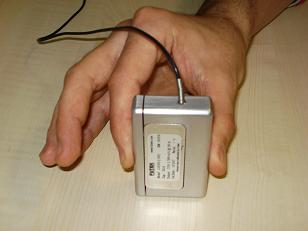
\includegraphics[height=0.16\textheight]{figs/grip1} &
    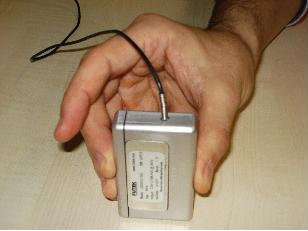
\includegraphics[height=0.16\textheight]{figs/grip2} &
    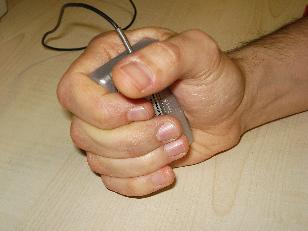
\includegraphics[height=0.16\textheight]{figs/grip3} \\
    $(a)$ & $(b)$ & $(c)$ \\
  \end{tabular}
  \caption{The three different grips employed in the experiment: $(a)$
   index precision grip; $(b)$ other fingers precision grip; $(c)$
   power grasp.}
  \label{fig:Grasps}
\end{figure*}

\begin{figure*}[!ht] \centering
  \begin{tabular}{cc}
    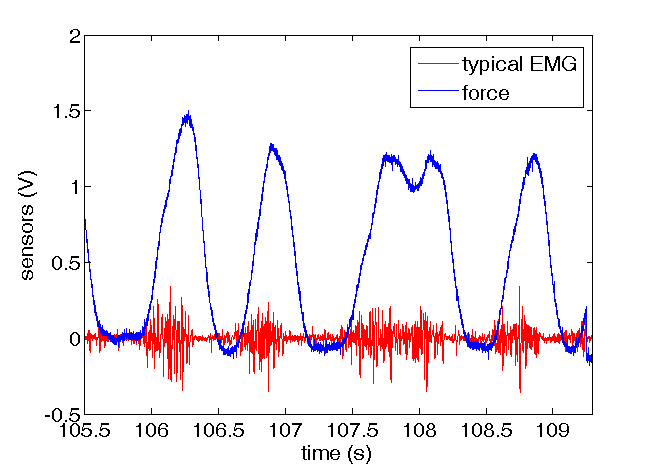
\includegraphics[width=0.45\textwidth]{figs/force_raw} &
    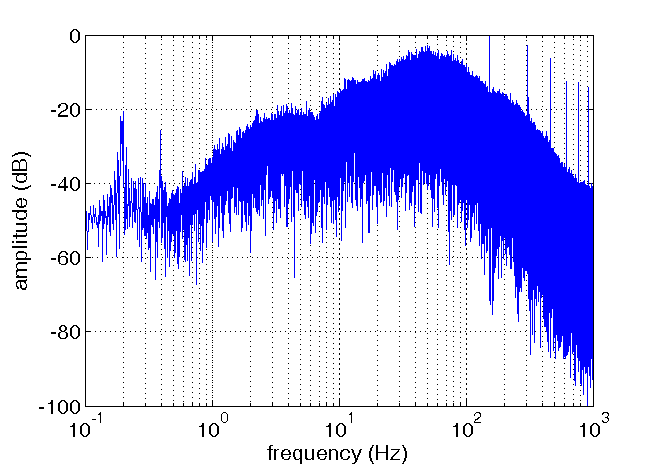
\includegraphics[width=0.45\textwidth]{figs/spectrum_raw} \\
    $(a)$ & $(b)$ \\
  \end{tabular}
  \caption{$(a)$ typical raw EMG and force signals; $(b)$ frequency diagram of
    the EMG signal.}
  \label{fig:spectra}
\end{figure*}

%During each phase,
The subject freely repeated each grasping action
for $100$'', resting for $30$'' in between grasps. In order to gather
more data and diminish the effect of local errors, the whole procedure
was repeated twice. As a whole, each subject's recording resulted in
about $2.4\times 10^6$ samples. 
%equally distributed in each phase.

Unlike commercial EMG electrodes, such as, e.g., Otto Bock's MyoBock
electrodes \cite{ottobock} that return the on-board computed Root-Mean
Square (RMS) of the EMG signal, the electrodes employed here return
the ``raw'' EMG signal.
% within 10Hz and 1kHz.
%without any low-pass filtering or Root-Mean Square (RMS) processing.
Nevertheless, it is well-known \cite{deluca,zecca} that the force
exerted by a muscle is strongly related to the RMS of the EMG signal,
rather than to the raw signal. For this reason, in order to have a
signal that is as similar as possible to a \emph{control signal}, we
decided to evaluate the RMS, electrode by electrode.

For a given mono-variate discrete time-varying signal, the RMS is
defined as the mean of the squares of the signal values, evaluated
over a certain time-window $T_{RMS}$. Roughly speaking, the RMS acts
like an envelope extraction plus a low-pass filter, whose cutoff
frequency grows smaller as the time-window grows larger (i.e., as
$T_{RMS}$ becomes higher). For this reason, high values of $T_{RMS}$
imply an ostensible delay in the resulting signal that is due to
\emph{responsiveness} of the synthesized output signal.  It becomes
slower and slower as the $T_{RMS}$ value increases, since more
``samples'' are averaged to obtain a significant value. The choice of
$T_{RMS}$ is therefore crucial to produce a signal which is maximally
related to the force signal, unaffected by high-frequency noise, and
with an acceptable lag. However, it must be noted here that the EMG
signal, being directly related to the muscle \emph{activation
potentials}, happens to \emph{anticipate} the muscle
movements\footnote{The electromechanical delay (EMD) of a muscle is
defined as the interval between the onset of the electrical activity
of the muscle (EMG) indicating its activation by the neural system and
the onset of the resulting change in the mechanical variable
observed. The delays reported range from 25 to 100ms for different
muscles and tasks \cite{Wolf1994}.}. Therefore, in practical
applications, it can be considered as acceptable a wider lag than what
one would expect.
%a wider lag is acceptable than one would expect. 
This is useful since it allows us to increase $T_{RMS}$, if necessary.

%\begin{figure*}[!ht] \centering
%  \begin{tabular}{ccc}
%    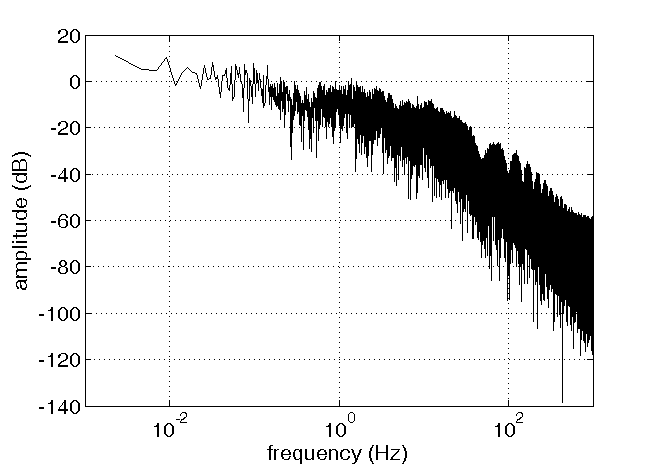
\includegraphics[width=0.3\textwidth]{figs/spectrum_RMS0040} &
%    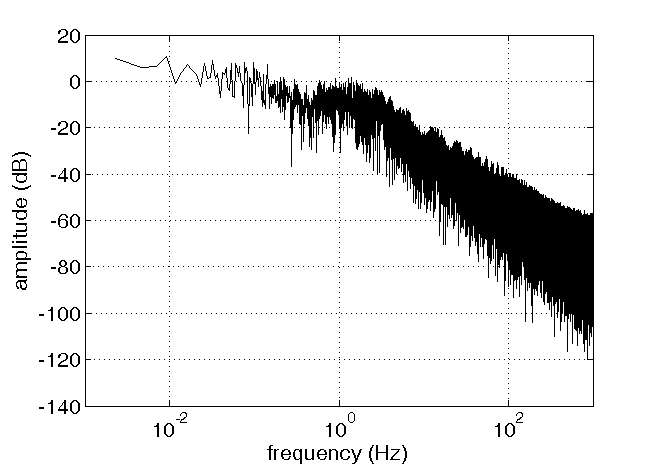
\includegraphics[width=0.3\textwidth]{figs/spectrum_RMS0200} &
%    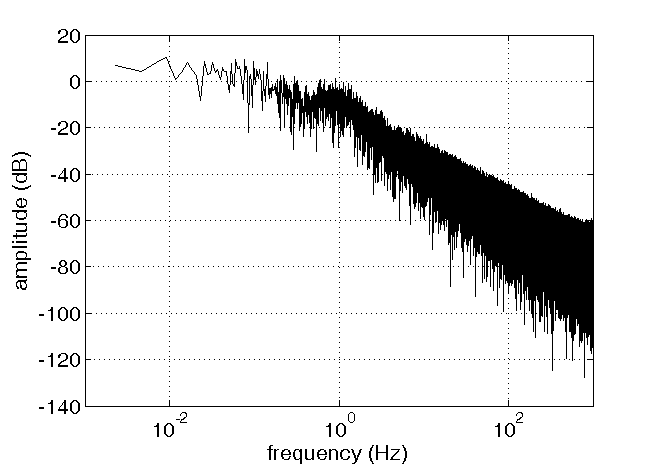
\includegraphics[width=0.3\textwidth]{figs/spectrum_RMS1000} \\
%    $(a)$ & $(b)$ & $(c)$ \\
%  \end{tabular}
%  \caption{(left to right) effects of the RMS on the bandwidth of the EMG
%    signals, for $T_{RMS} = 20, 100, 500ms$.}
%  \label{fig:RMSs}
%\end{figure*}

%Unfortunately 
We are not aware of any systematic way of setting a good value of
$T_{RMS}$ in such a framework. Therefore we found $T_{RMS}$
heuristically, according to some initial experiments.
% As an example, though, consider Figures \ref{fig:spectra} and \ref{fig:RMSs}.

Figure \ref{fig:spectra} (panel $(a)$) shows a few seconds of typical
force/EMG behavior: it is apparent that the EMG signal starts oscillating when the force signal
starts increasing. It is also quite clear that the
amplitude of the envelope of the EMG is related to the force, as
indicated in the literature. Panel $(b)$ shows the frequency analysis
of the same EMG signal: as one can see, the meaningful bandwidth lies
in the interval known from the literature.

%On the other hand, Figure \ref{fig:RMSs} shows the effect of the RMS on the frequency components of the EMG, for three different values of $T_{RMS}$.
%It is clear that the meaningful bandwidth now contains all low-frequency components, possibly down to the constant, and is upper-bounded by about $25$Hz (panel $(a)$, for $T_{RMS}=20ms$) to $10$Hz (panel $(c)$, for $T_{RMS}=0.5s$). As expected, larger values of $T_{RMS}$ correspond to a better filtering but also to a larger delay.

This enables us to safely sub-sample the EMG signal after having
applied the RMS. Assuming that $T_{RMS}$ is not too small, we
subsampled both the EMG and force signal at $25$Hz, taking one sample
every $80$ of the original sequence.  This considerably reduced the
amount of data to be processed, namely to about $30.000$ samples for
each subject.

As a last data pre-processing step, we removed from the sample set
those samples for which the applied force was lower than a specific
threshold, in order to get a clearer representation of the activation
potentials. This threshold was chosen in order to remove a minimal
fraction of the samples. Of course, we fully retained the samples
corresponding to the baseline rest condition.  This is why we chose to
record this condition before the data acquisition.
%rest of the experiment.


\section{Data Pre-processing and Preliminary Analysis}
\label{sec:pre}
The data related to each subject and modality were chronologically
juxtaposed exactly in the order the experiments were performed; then a
label was attached to each sample, according to the type of grasp
required from the subject. Samples associated with a low force value
were given the label $0$, since they denote no activity of the
muscles, that is, a resting condition. Subject $1$ actually needed the
no-action data set to be replicated for each modality, since we did
not record its baseline each time --- a mistake which was corrected
with the second and third subject. Moreover, we could not record the
"pointing index" activity for this subject in the second modality,
which is therefore null.

\begin{figure*}[!ht] \centering
  \begin{tabular}{ccc}
    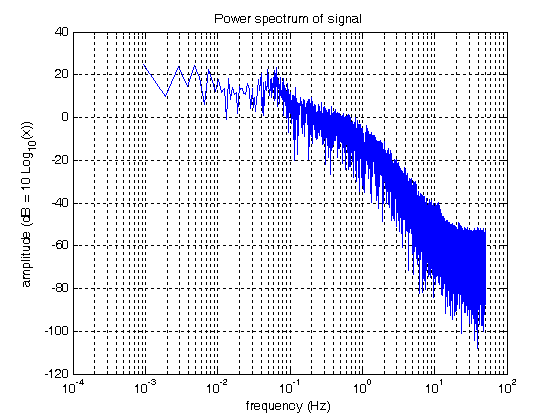
\includegraphics[width=0.3\textwidth]{figs/spectrum_force} &
    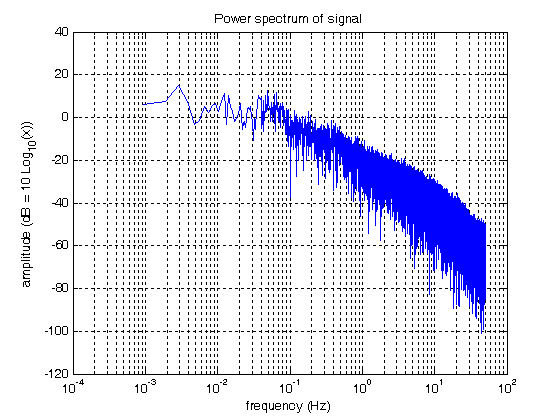
\includegraphics[width=0.3\textwidth]{figs/spectrum_electrode_1} &
    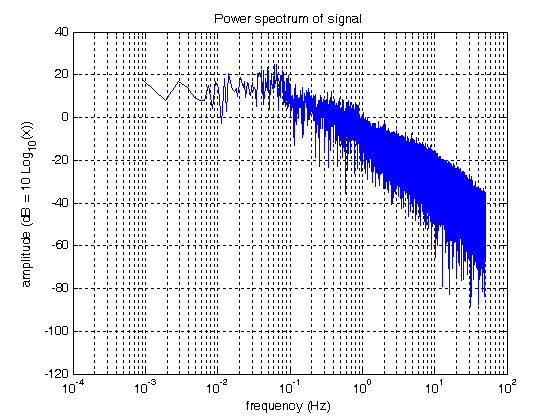
\includegraphics[width=0.3\textwidth]{figs/spectrum_electrode_3} \\
    force & electrode $1$ & electrode $3$ \\
  \end{tabular}
  \caption{frequency analysis of the force signal and two
    typical electrodes.}
  \label{fig:spectra}
\end{figure*}

Spectral analysis of the EMG signal as read from the electrodes, in
agreement with the literature, shows that its relevant bandwidth lies
below $10$-$12$Hz (see Figure \ref{fig:spectra}), so we could safely
subsample the signals at $25$Hz, that is, considering one sample in
four of the original data stream. This made the data set to be dealt
with much smaller and computationally tractable. Subsequently, we
applied a II order low-pass filter with cutoff frequency at $5$Hz in
order to remove all possible high-frequency noise. This has proved to
be a very effective way of getting a good signal in early experiments
(see \cite{2008.Neurorob}).

Principal Component Analysis (PCA) reveals that the 5 signals can be
linearly reduced to two losing, on average, only $7.7\% \pm 4.4\%$ of
the signal variance; therefore, we can visualise the samples, tagging
them according to the labels (and therefore according to the action)
and visually detecting how well the subjects can produce different EMG
patterns when they are asked to simulate different grasping
actions. Figure \ref{fig:PCA} shows the results, according to each
subject and modality.

\begin{figure*}[!ht] \centering
  \begin{tabular}{ccc}
    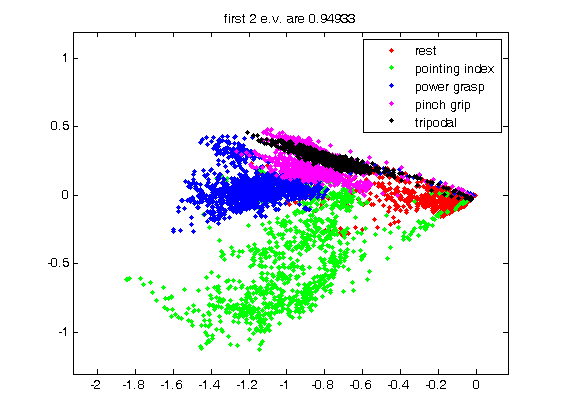
\includegraphics[width=0.3\textwidth]{figs/data11} &
    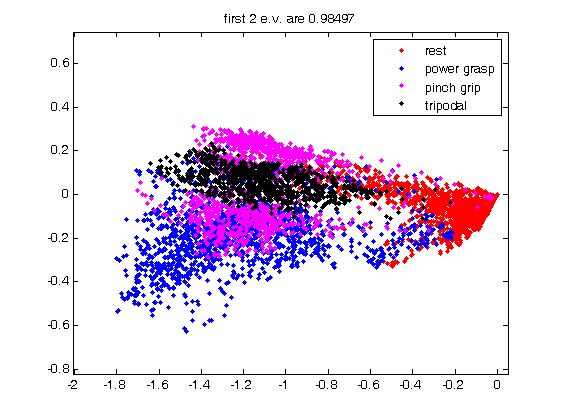
\includegraphics[width=0.3\textwidth]{figs/data12} &
    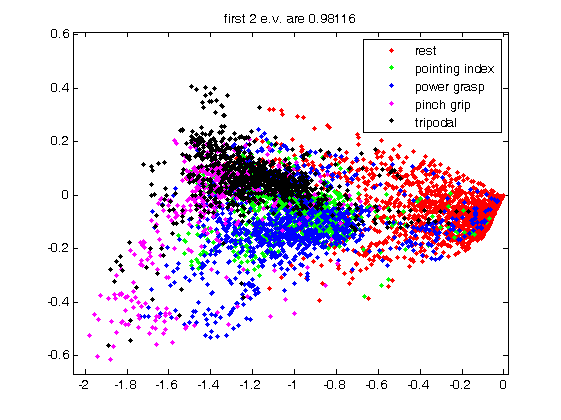
\includegraphics[width=0.3\textwidth]{figs/data13} \\
    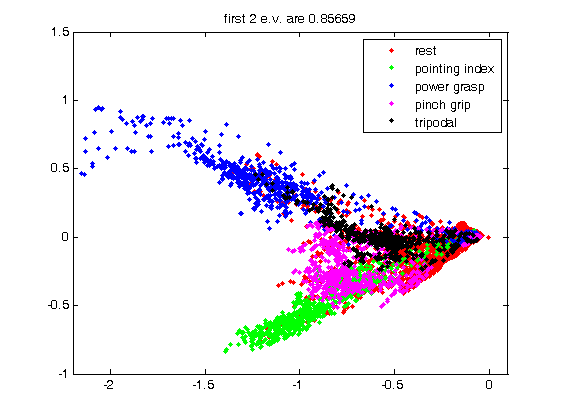
\includegraphics[width=0.3\textwidth]{figs/data21} &
    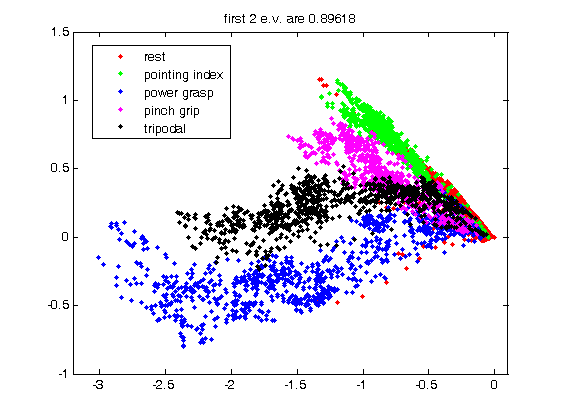
\includegraphics[width=0.3\textwidth]{figs/data22} &
    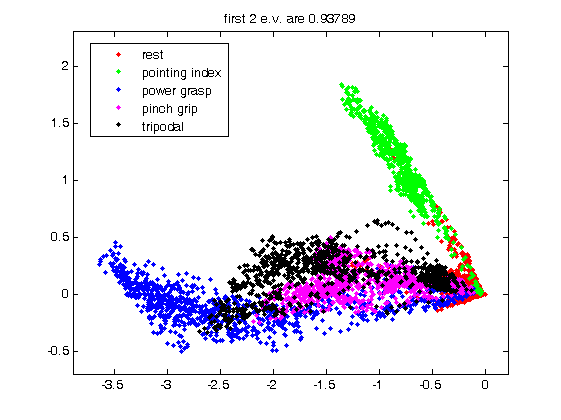
\includegraphics[width=0.3\textwidth]{figs/data23} \\
    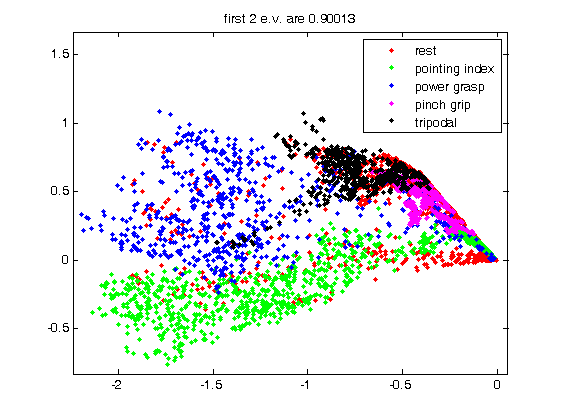
\includegraphics[width=0.3\textwidth]{figs/data31} &
    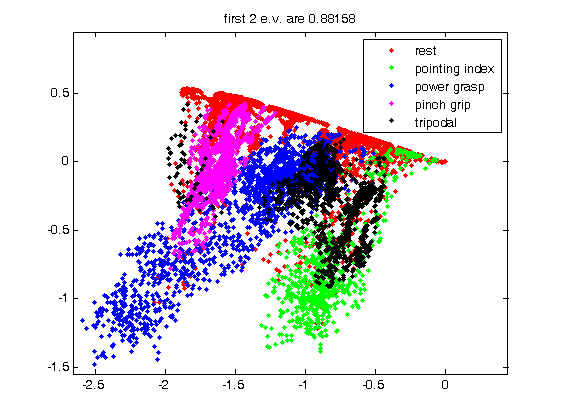
\includegraphics[width=0.3\textwidth]{figs/data32} &
    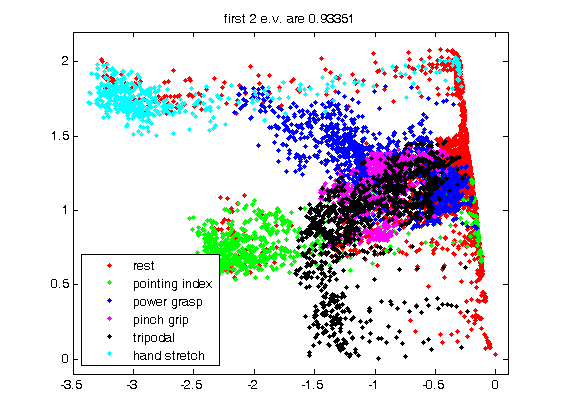
\includegraphics[width=0.3\textwidth]{figs/data33} \\
  \end{tabular}
  \caption{ PCA analysis of the subjects' data. (top to bottom)
    Subject $1$, $2$ and $3$; (left to right) modality $1$, $2$ and
    $3$. Notice that subject $1$, modality $2$ has no ``pointing
    index'' data, and that subject $3$ has the ``hand stretch'' data.}
  \label{fig:PCA}
\end{figure*}

As is apparent from the Figure, all subjects can produce remarkably
well separated and distinct signals, according to the elicited type of
grasp. In particular, notice how two very similar grasp types, i.e.,
pinch grip (thumb and index come together as to precisely grip, e.g.,
a pen) and tripodal grip (the same, but done with the middle finger,
too) appear well separated on almost each graph --- look at the black
and pink coloured samples.

Notice, as well, that the graphs have not all the same scale and that
they appear incongruent with one another, but this is due to $(a)$
having positioned the electrodes irrespective of their order number on
the stumps of the patients; and $(b)$ the PCA coefficients being
evaluated in a blind way. This problem seems, anyway, ininfluent on
the result of the experiment, since a machine learning approach such
as SVMs is supposed exactly to automatically find patterns and
regularities among the samples for each subject.

One last point is that PCA being so effective in reducing the
dimensionality of our data to two does not necessarily imply that we
could use two electrodes only to obtain the same results; this depends
on the PCA coefficients, which show consistently the same magnitude
(except in the case of subject $3$, where a heavy drift was observed
on two electrodes, very likely due to sweating --- this is a well-known
problem of EMG-controlled prosthetics). This means that each electrode
is required to give a uniformly-weighted contribution to the
PCA-transformed $2$-dimensional samples. Of course reducing the
required number of electrodes is a requirement, since this would make
the prosthesis cheaper. We are invesitigating the issue.


\section{Results}
\label{sec:exp}
\section{Results}
\label{sec:exp}

Figure \ref{fig:results} shows the performance results obtained by the SVMs
in classification and regression for each subject and modality; Figure
\ref{fig:guess} shows four examples of predicted targets.

\begin{figure*}[!ht] \centering
  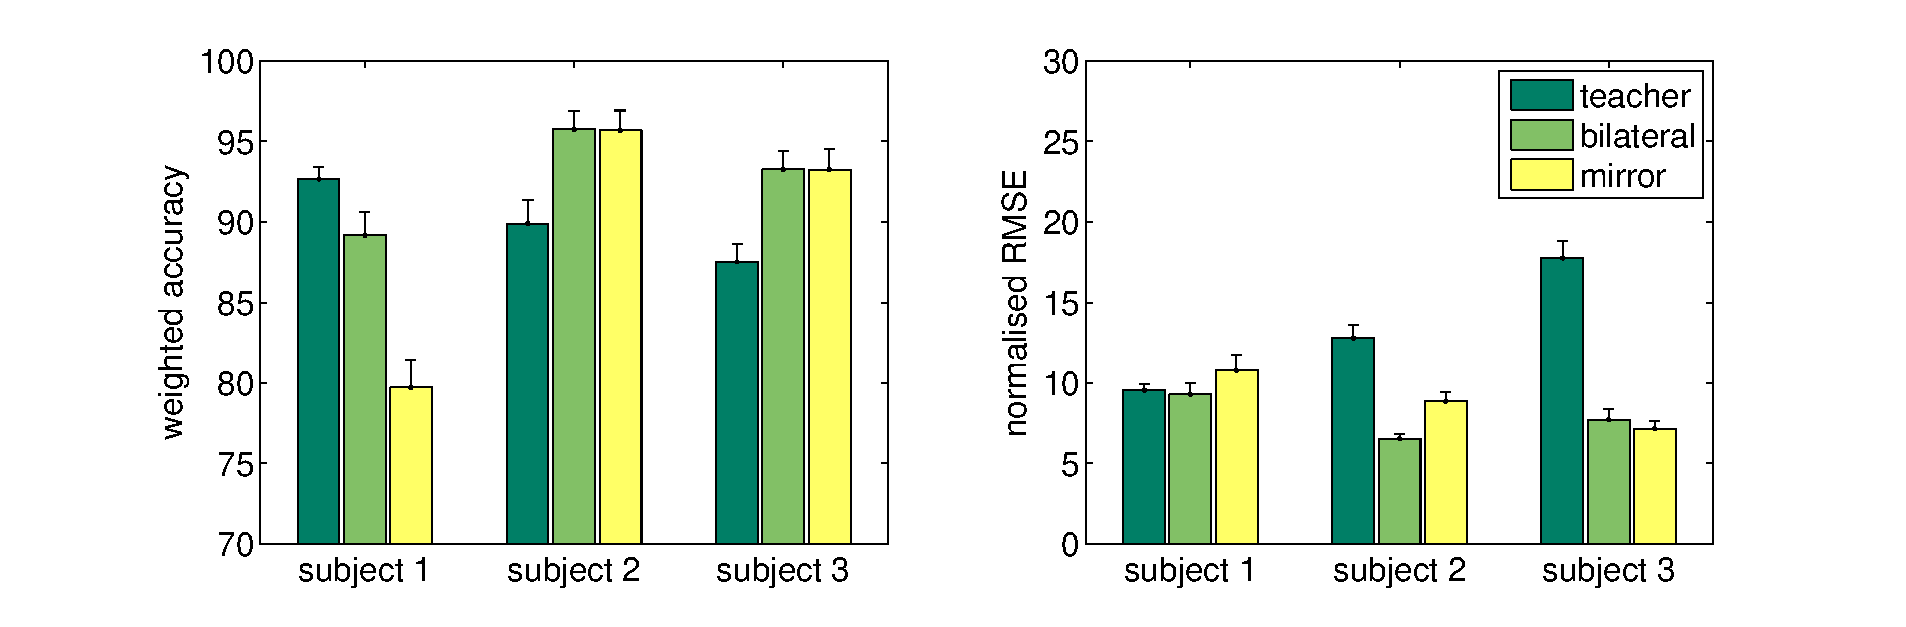
\includegraphics[width=\textwidth]{figs/figPerf}
  \caption{classification (left) and regression (right) performance
    for each subject and modality. Histogram bars are mean values over
    the $10$ splits of the outer cross-validation, error bars denote one
    standard deviation.}
  \label{fig:results}
\end{figure*}

Classification performance ranges from $95.74\% \pm 1.15\%$ (Subject $2$,
bilateral action) to $79.72\% \pm 1.70\%$ (Subject $1$, mirror-box). Highest
performances per subject are $92.67\% \pm 0.74\%$ (Subject $1$ in teacher
imitation modality), $95.74\% \pm 1.15\%$ (Subject $2$, bilateral action)
and $93.26\% \pm 1.11\%$ (Subject $3$, bilateral). Notice that
bilateral action and mirror-box are not significantly different as far as
Subjects $2$ and $3$ are concerned. A definite descending trend is observed
for Subject $1$ from imitation to bilateral to mirror-box, while this trend
is reversed for Subjects $2$ and $3$, which perform much better in the last
two modalities than in the first one. Modality-wise, teacher imitation is
the best modality for Subject $1$, while the other two are best for Subjects
$2$ and $3$.

Regression performance\footnote{Notice that the regression performance index
is an \emph{error}, while the classification performance is an \emph{accuracy};
therefore in the case of classification, the higher the bars, the better, whereas
it is the other way around in regression.} ranges from $6.54\% \pm 0.31\%$ (Subject $2$,
bilateral) to $17.76\% \pm 1.06\%$ (Subject $3$, teacher). Subject $1$ has
little or no significative difference among modalities, obtaining the best
performance while doing bilateral action ($9.29\% \pm 0.73\%$); Subject $2$
is best in bilateral action ($6.54\% \pm 0.31\%$) while Subject $3$ performs
best in mirror-box ($7.17\% \pm 0.43\%$) with high overlapping with the bilateral
modality. Subject-wise, Subjects $2$ and $3$ perform remarkably bad in teacher
imitation modality if compared with the other two; while modality-wise, we here
notice again that teacher imitation gets worse and worse as we move from Subject
$1$ to $2$ to $3$. A reversed trend is almost consistently observed for the other
two modalities.

\begin{figure*}[!ht] \centering
  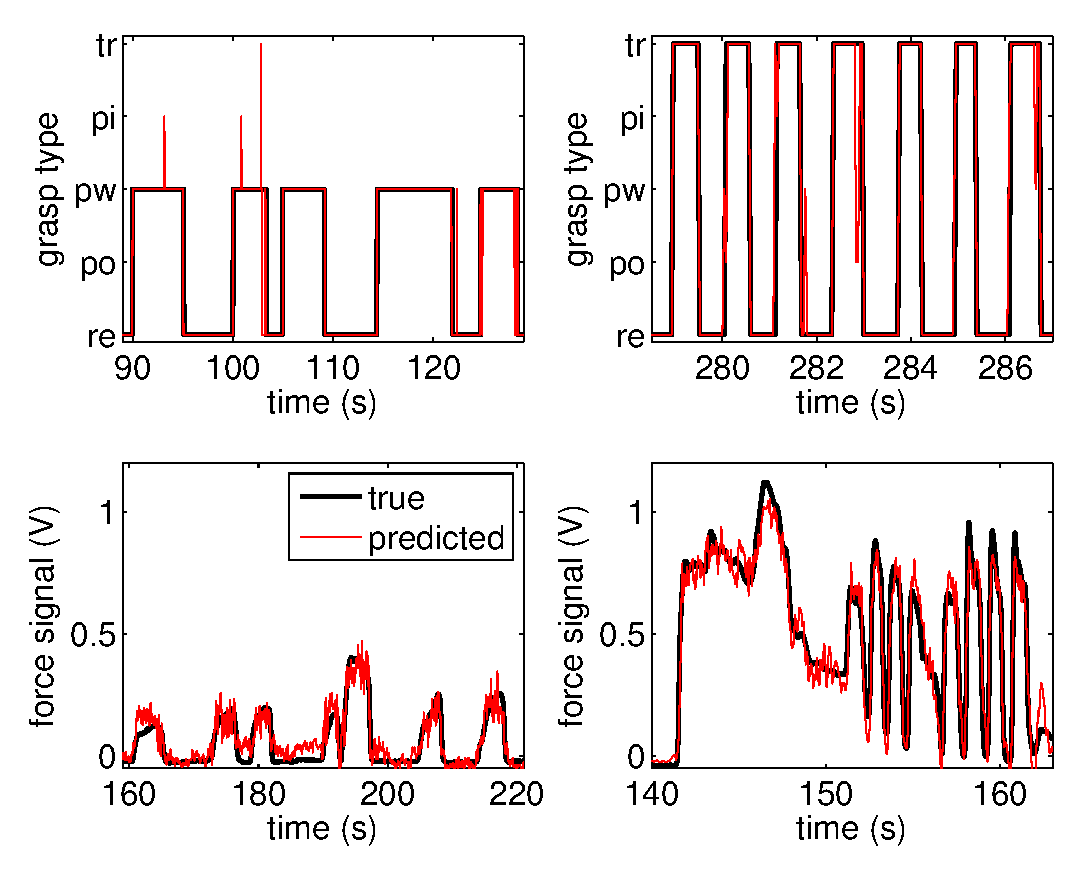
\includegraphics[width=\textwidth]{figs/figGuess}
  \caption{comparing true and predicted targets. (upper row) Classification
    of Subject $2$ in bilateral action (left, weighted accuracy $95.74\% \pm
    1.15\%$) and Subject $1$ in mirror-box (right, $79.72\% \pm 1.70\%$).
    (lower row) Regression of Subjects $2$ (left, normalised RMSE $6.54\% \pm
    0.31\%$) and $3$ (right, $7.70\% \pm 0.65\%$) in bilateral action.}
  \label{fig:guess}
\end{figure*}

Figure \ref{fig:guess} indicates that (upper row) most errors in classification
appear at the onset of grasps (transitions to/from label \re), although for Subject $1$
\pw\ and \pi\ are also frequently mistaken. Regression (lower row) appears good
both when force is approximated during slow (left panel) and fast (right panel)
grasps. The only significant disturbance is a high-frequency but low-amplitude
modulation of the predicted force. Confusion matrices for each subject and
modality (Figure \ref{fig:confusion}) actually confirm that \re\ is easily mistaken
for any other label (first row and column of each matrix), in particular for
Subjects $2$ and $3$. Subject $1$ has a more complex schema of label confusion,
depending on the modality. In particular, during teacher imitation, \pi\ and
\tr\ are easily confused; during bilateral action, \pi\ and \pw\ are as well
confused; and in mirror-box modality the pointing index and the power grasp
are those most easily mistaken. Actually, this is qualitatively confirmed by
considering again the PCA-reduced sample scatterplots of Figure \ref{fig:PCA},
first row.

\begin{figure*}[!ht] \centering
  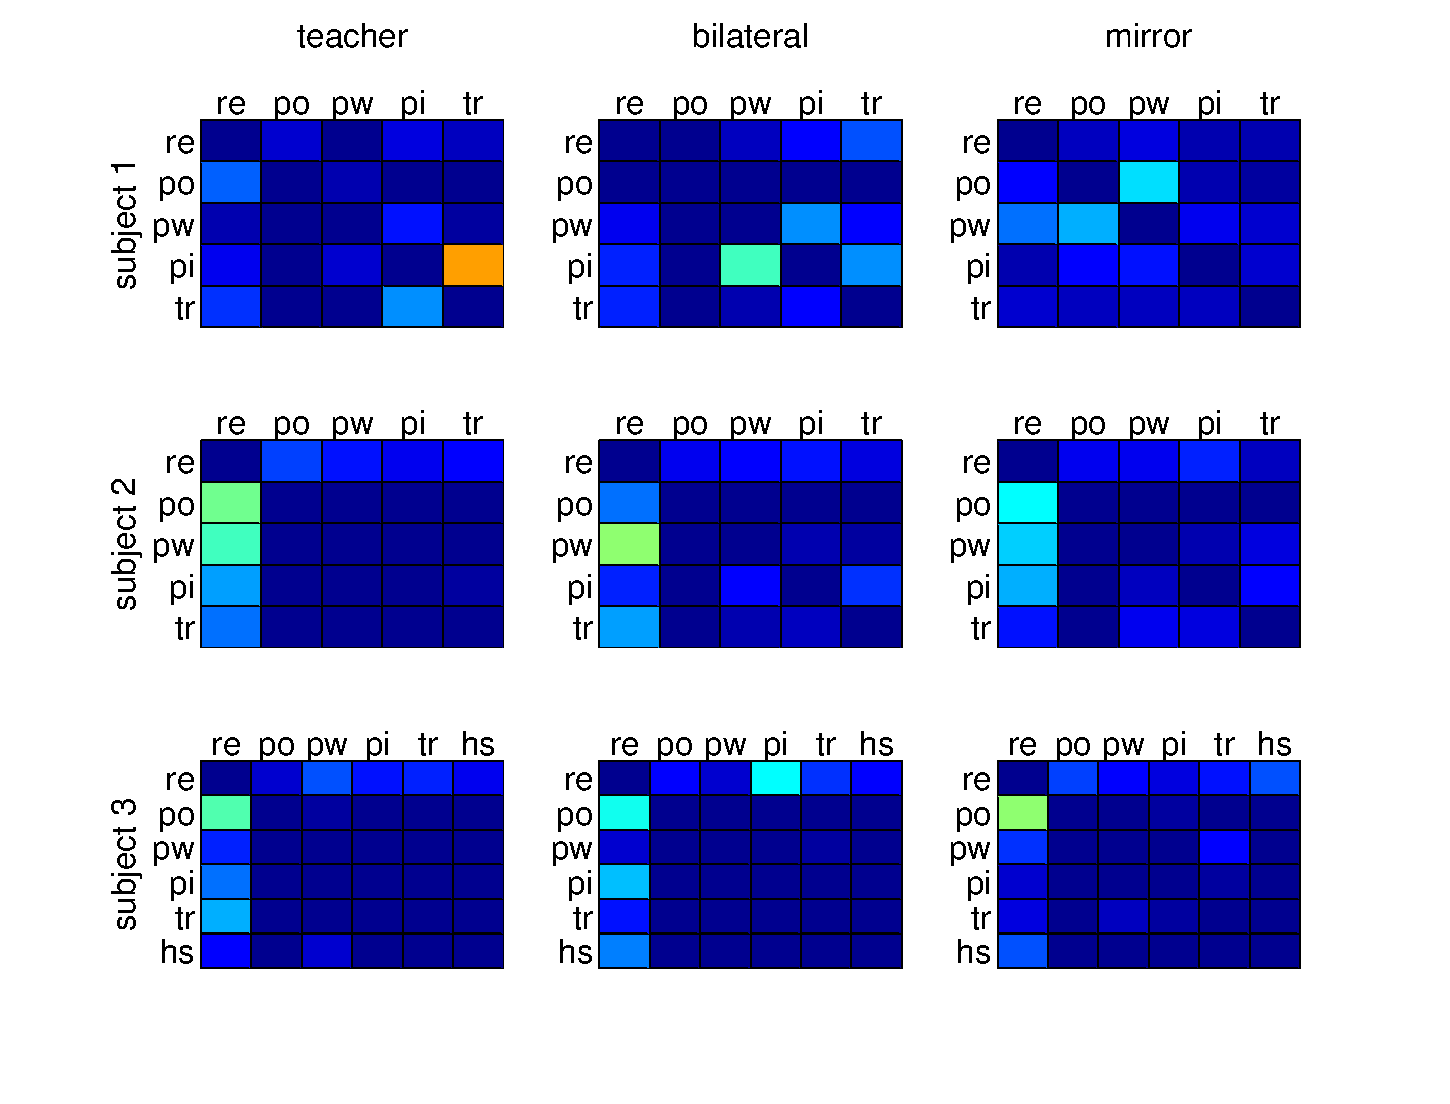
\includegraphics[width=\textwidth]{figs/figConf}
  \caption{confusion matrices for each subject and modality.
    In each matrix $C$, $C_{ij}$ denotes the fraction of labels
    $i$ which have been mistaken for $j$ over the total mistaken
    labels of that particular cycle. The diagonals of the matrices
    are obviously identically zero. Each matrix is the average of
    ten matrices, obtained from each outer cross-validation split.}
  \label{fig:confusion}
\end{figure*}

Lastly, Figure \ref{fig:SVs} shows the percentages of SVs for each
subject and modality, for the optimal models both for classification
and regression. Comparing this Figure with Figure \ref{fig:results},
an almost uniform inverse correlation is apparent,
between performance and percentage of SVs, as predicted.
Lowest percentages of SVs per subject in classification models are
$19.73\% \pm 4.10\%$ (Subject $1$, teacher imitation),
$24.59\% \pm 0.22\%$ (Subject $2$, bilateral action), and
$15.83\% \pm 1.36\%$ (Subject $3$, bilateral action again).
For regression, we have
$12.98\% \pm 0.19\%$ (Subject $1$, teacher imitation),
$8.28\% \pm 0.32\%$ (Subject $2$, bilateral action), and
$9.97\% \pm 0.13\%$ (Subject $3$, bilateral action once again).

\begin{figure*}[!ht] \centering
  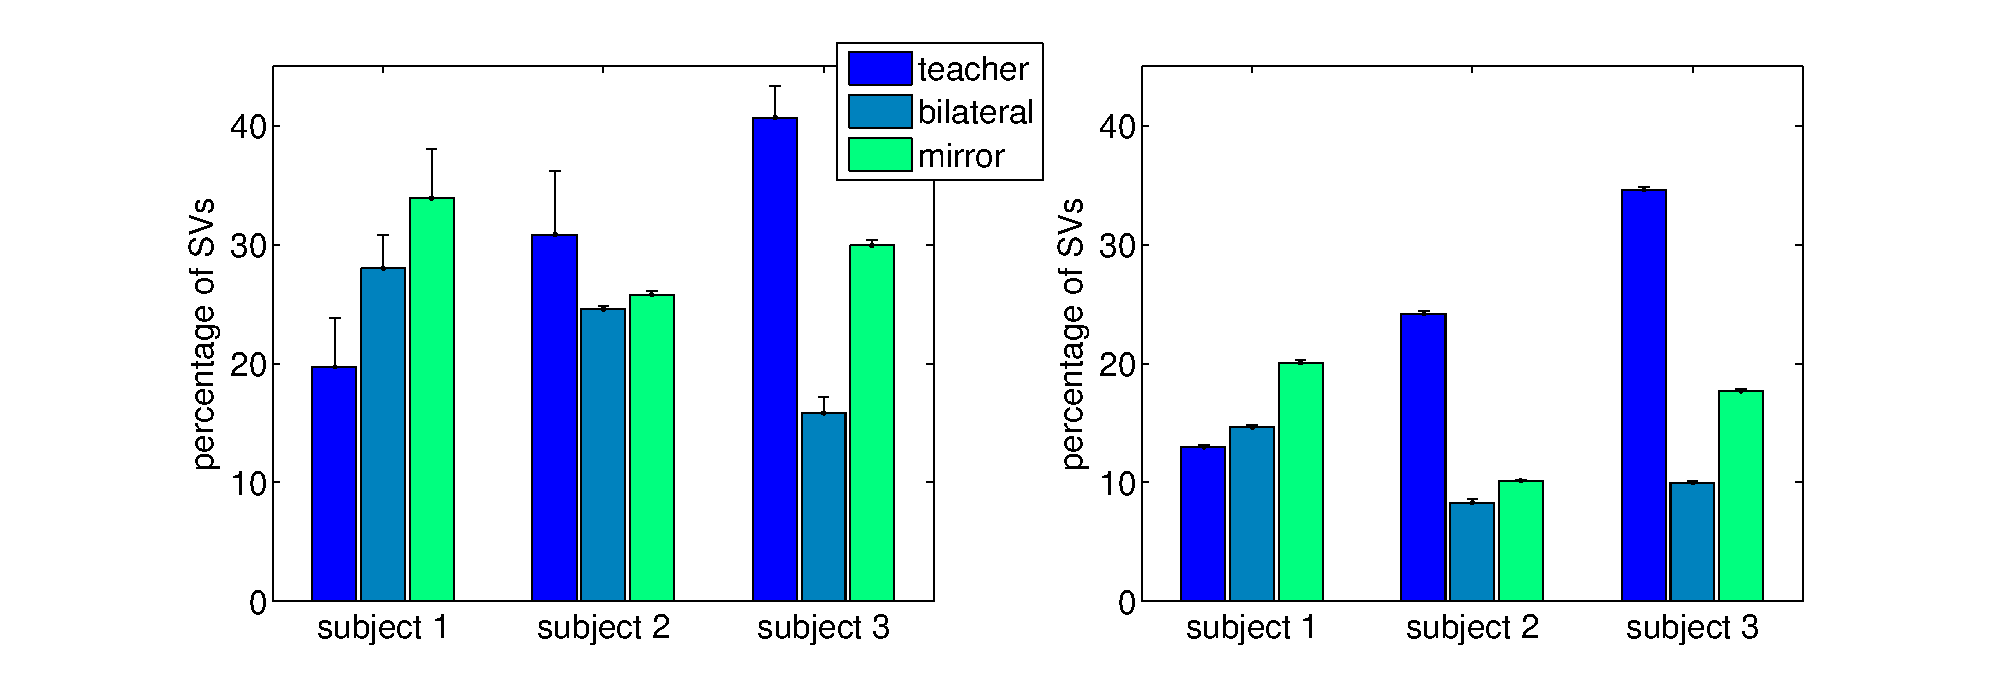
\includegraphics[width=\textwidth]{figs/figSVs}
  \caption{percentages of Support Vectors obtained in the optimal models
  	for classification (left) and regression (right) for each subject and modality.
    Histogram bars are mean values over the $10$ splits of
    the outer cross-validation, error bars denote one standard deviation.}
  \label{fig:SVs}
\end{figure*}


\section{Discussion and Conclusions}
\label{sec:disc}
The results hereby presented clearly show that the plain, old EMG
signal can be used to drive a mechanical hand / prosthetic hand in a
radically new way: finer, force-controlling, more dexterous. Our
results indicate that a machine learning approach such as Support
Vector Machines will effectively detect well-separated grasping
patterns in real time, as required by an amputee; at the same time,
the system will be able to detect how much force is involved in the
grasp. If the prosthesis has a sufficient number of DOFs, that is, it
can be position-controlled to mimic the required grasps, and if it can
be force-controlled, then our system will be able to control it in a
totally natural way, that is, according to what the patient wants it
to do.

The positioning of the electrodes, at least in the case of the three
patients who joined the experiment, is uniform and not related to any
anatomical consideration. Since the results we have obtained are
uniformly good for all patients, it is probably possible to claim that
careful positioning, as well as medical control to identify the best
working remaining muscles in the stump, is not required. This would
simplify the whole procedure.

The proposed analysis of SVM hyperparameters and percentage of Support
Vectors with respect to the total number of training samples (see
Section \ref{sec:exp}) indicates that the problem is rather easy, if
considered form the pure point of view of machine learning. This lets
us hope that, in case SVMs proved too hard to implement in practice,
even a less sophisticated method such as, e.g., nearest neighbours,
could obtain acceptable performance values. Anyway, our realistic
implementation analysis shows that there should be no problem in
miniaturising the system, and embedding it in a prosthesis, even a
commercially available one.

As far as training is concerned, it is worth noting that soon on-line
learning could be needed, especially since patients are not supposed
to remain in controlled conditions while wearing the prosthesis. In
previous or submitted work, we have already shown that the framework
is theoretically perfectly able to work in non-controlled conditions
(the so-called Daily-Life Activity analysis). As well, it has been
shown that a sparsification strategy such as \emph{uniformisation} can
enforce on-line learning of new situations at the price of degrading
the performance reasonably. It remains to adapt the proposed PC /
microcontroller architecture to such a continual retraining schema,
but this seems no big problem.

Lastly, a few notes from a rather medical point of view. In this work
we are making \emph{no statement at all} about the physiological
resemblance of the patterns we deal with, with respect to the muscular
patterns elicited for the same grasps in a healthy arm. Actually, we
have not investigated what the patient's stump muscles do when the
patient is asked to imagine, e.g., a pinch grip --- this is indeed a
very interesting issue, but is not the focus of this work. Since each
and every amputation is different from one another, and therefore each
stump has different muscular conditions, what we can hope for is that
the system works fine for a reasonable range of amputees and
stumps. Although we have only $3$ patients here, their diversity as
far as age, age of operation and type of amputation lets us hope for
the best. In the end, as long as for each patient, each grasp type or
posture corresponds to a different pattern, then we can detect it and
send the appropriate command to the prosthesis. The patient will then
be able to elicit from the prosthesis, say, a $5$N pinch grip, or a
$30$N power grasp, just by ``desiring'' so. This is what we mean by a
better quality of life for amputees and a shorter training time. The
keyword \emph{adaptive prosthetics} is meant, here, in the
machine-learning sense, that is: the prosthesis is trained upon the
patient's data and therefore adapts to her/him.

We have actually found it surprising that so much fine muscular
activity can be elicited from elderly patients, such as our subjects
$1$ and $2$, who, by the way, have been operated \emph{decades}
ago. Notwithstanding this, they are still perfectly able to produce,
e.g., two very different patterns for similar grips such as the index
/ thumb pinch grip and the tripodal grip. This lets us hope that
possibly even a simpler method than SVMs could be used without
degrading the performance too much, in case the miniaturisation of
this method proves too hard in practice. But actually, the analysis
performed in Section \ref{sec:impl} is very promising.

The use of three different modalities has proven effective in finding
the best way for each single patient to train the system. Actually, as
one can see by considering Table \ref{tab:results} again, subject $1$
obtains better results if he trains the system in the teacher
imitation modality, whereas subjects $2$ and $3$ make it work better
in the bilateral action and mirror-box modalities. It is unclear why
this is the case, and anyway a broader range of patients is required
to observe any stastically meaningful phenomenon, in order to possibly
relate the type of amputation to the preferred modality --- a
relationship which would be of great help when a new patient has to
train the system. Here we can note that subject $1$ is the one left
with the shortest stump. One possibility why he performs best in the
teacher imitation modality is then\footnote{personal communication
with Benoni B. Edin of the Ume\o a University, Sweden.\textbf{FIXME}}
that he presents the ``highest degree'' of de-afferentiation in his
forearm, since he misses most of it, as opposed to subjects $2$ and
$3$. Literature on de-afferentiated patients (see, e.g.,
\cite{...}) indicates that such a condition, at least in neuropathic
patients, eases tasks in which motor and visual perception are
de-coupled or contradictory; and this seems to be the case, since
subject $1$ obtains better results when he has to \emph{imitate
someone else} rather than figuring out his own movements.


\section*{Acknowledgments}

The authors would like to thank Mr. Cesare Stagni of INAIL Centro
Protesi for kindly helping us finding the patients who have joined the
experiment. We also thank Benoni B. Edin of Ume\aa\ University,
Sweden, for a helpful comment on the paper.

\bibliographystyle{elsarticle-harv}
\bibliography{paper,../../claudio}

\end{document}
